\section{Derivative}
The partial derivative of $f$ with respect to the $i$-th coordinate function is defined through
\[
\frac{\partial}{\partial x_i}f(x) = \lim\limits_{x\rightarrow 0}\frac{(x + t\cdot \vec{e}_i) - f(x)}{t}
\]
The \textbf{gradient} of $f$ as $n$-dimensional row vector, whose components correspond to the various partial derivatives
\[
\nabla f(x) = \left(\frac{\partial}{\partial x_1}f, \frac{\partial}{\partial x_2}f \dots \frac{\partial}{\partial x_n}f\right)
\]

\noindent\textbf{Example:} $f(g) = \cos(g); \qquad g(x) = e^{2x}$ \\\indent \textbf{Partial}:
\begin{align*}
	\frac{\partial f}{\partial x} = -\sin(g) \\
	\frac{\partial g}{\partial x} = 2e^{2x}
\end{align*}
\indent \textbf{Total}
\begin{align*}
	\frac{df}{dx} = \frac{df}{dx}f(g(x)) = -\sin(e^{2x})e^{2x}
\end{align*}


\subsubsection{Properties}
\begin{align*}
	\nabla(f \pm g) &= \nabla f \pm \nabla g \\
	\nabla(f \cdot g) &= g\nabla f + f\nabla g \\
	\nabla\frac{f}{g} &= \frac{g\nabla f - f\nabla g}{g^2} \\
	\nabla\left|\mathbf{r}\right| = \nabla \sqrt{\sum_{i = 1}^{n}r^2_i}  &= \frac{\mathbf{r}^T}{\left|\mathbf{r}\right|}
\end{align*}



\subsection{Chain Rule}
\begin{center}
	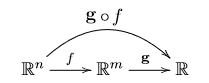
\includegraphics[width=0.4\columnwidth]{Images/screenshot001}
\end{center}
Jacobian $\mathbf{J}_{\vec{g}\circ\vec{f}}$ can be calculated by using the chain rule, whenever $\mathbf{J}_{\vec{g}}$ and $\mathbf{J}_{\vec{f}}$ already given:
\[
\mathbf{J}_{\vec{g}\circ\vec{f}}(t) = \mathbf{J}_{\vec{g}}(t)\cdot\mathbf{J}_{\vec{f}}(t)
\]
Alternative spellings:
\begin{align*}
	\frac{\partial}{\partial t}f(t) = \frac{\partial}{\partial f}g(f(t)) \cdot \frac{\partial}{\partial t}f(t)
\end{align*}
For 1 Dimension:
\[
\frac{d}{dt}g(f(t)) = \mathbf{J}_{\vec{g}\circ\vec{f}}(t) = \nabla g(f(t)) \cdot \vec{f}(t)'
\]

\subsection{Jacobian Matrix}
Jacobian-Matrix is a matrix of all it's first order partial derivatives. In case of \textbf{total derivates} the matrix is an approximation if $f$. It can also be used for minimizing multi-dimensional functions.
\[
\mathbf{J}_{\vec{f}}(\vec{x}_0) = \frac{d}{dx}\vec{f}(x) = \nabla\vec{f} = \begin{pmatrix}
	\frac{\partial f_1}{dx_1} & \dots & \frac{\partial f_1}{dx_n} \\
	\vdots & \ddots & \vdots \\
	\frac{\partial f_m}{dx_1} & \dots & \frac{\partial f_m}{dx_n} \\
\end{pmatrix} \qquad \in \mathbb{R}^{m \times n}
\]
\noindent\textbf{Note:} For more complicated excersices also the chain rule can be used.

\subsection{Liniarisation}
\[
\vec{f}(\vec{x}) \approx \vec{f}(\vec{x_0}) + \mathbf{J}_{\vec{f}}(\vec{x}_0) \cdot (\vec{x} - \vec{x}_0)  \qquad \vec{x} \approx \vec{x}_0
\]
\textbf{Note:} If there is no $\vec{x}_0$ available, we can define own. For example $x(1.1, 0.1, -0.9)$ is approximately $x_0(1, 0, -1)$

\subsection{Affine Transformation}
Affine Transformation are linear functions with bias, the jacobian matrix $\mathbf{J}_A$ for those arbitrary matrix $M$ is also known as:
\[
\mathbf{A}(x) = \mathbf{M}\mathbf{x} + \mathbf{b} \xRightarrow[]{!} \nabla \mathbf{A}(x) =  \mathbf{J}_A(x) = \mathbf{M}
\]
